%%Énoncé
Faites une liste exhaustive des différents cas qui peuvent se présenter lorsque l’on
ajoute un élément dans un arbre AVL et indiquez dans chaque cas la technique de
rééquilibrage utilisée (vue comme une ou plusieurs rotations). Complétez pour ce
faire les cas décrits en annexe de ce document. (Tanguy) \footnote{Les figures sont issues de DSAJ-5 p448}
\\
%%Réponse
Cas 1: Rééquilibrage par simple rotation
\begin{figure}[!h]
	\centering
	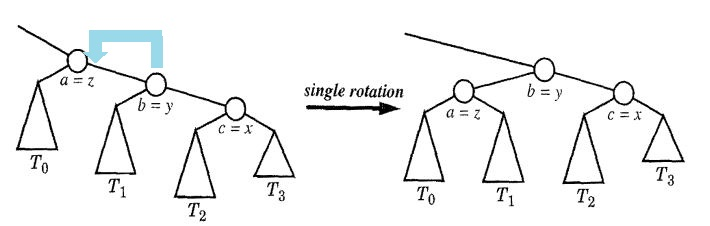
\includegraphics[scale=1]{q7-b1.jpg}
	\label{fig:equi}
\end{figure}
\\
\begin{figure}[!h]
	\centering
	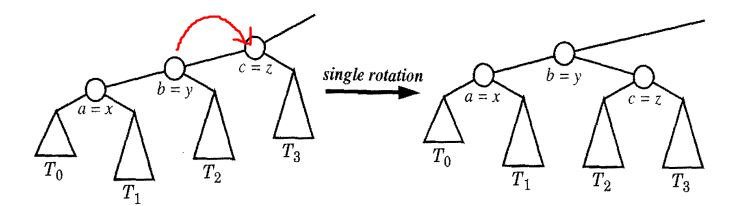
\includegraphics[scale=1]{q7-b2.jpg}
	\label{fig:equi}
\end{figure}
\\
Cas 2: Rééquilibrage par double rotation
\begin{figure}[!h]
	\centering
	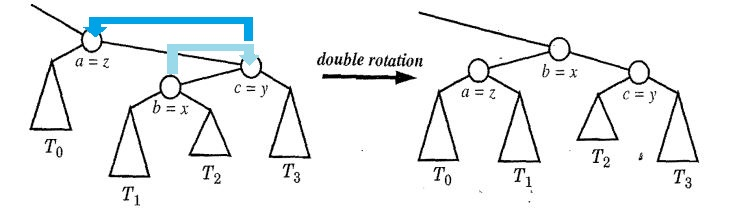
\includegraphics[scale=1]{q7-b3.jpg}
	\label{fig:equi}
\end{figure}
\\
\begin{figure}[!h]
	\centering
	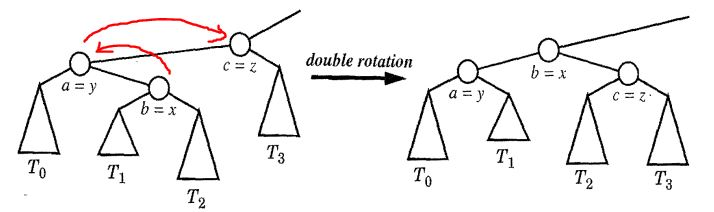
\includegraphics[scale=1]{q7-b4.jpg}
	\label{fig:equi}
\end{figure}